\documentclass[conference]{IEEEtran}
\IEEEoverridecommandlockouts
% The preceding line is only needed to identify funding in the first footnote. If that is unneeded, please comment it out.
% \usepackage{cite}
\usepackage{amsmath,amssymb,amsfonts}
\usepackage{algorithmic}
\usepackage{graphicx}
% \usepackage{textcomp}
\usepackage{xcolor}
\usepackage{booktabs}
\usepackage{multirow} 
\usepackage{url}
\usepackage{listings}
\usepackage{array} % Required for column width adjustments
\usepackage{tabularx}
\usepackage{balance}
\usepackage{colortbl} 
% \usepackage{footnote}
\usepackage{natbib} 
\usepackage{adjustbox}
\usepackage{makecell}
\usepackage{hyperref}

\def\BibTeX{{\rm B\kern-.05em{\sc i\kern-.025em b}\kern-.08em
    T\kern-.1667em\lower.7ex\hbox{E}\kern-.125emX}}
\begin{document}

\title{
LLMs at the Edge: Performance and Efficiency Evaluation with Ollama on Diverse Hardware
}

% \author{Anonymous Submission}

% \iffalse
% \author{\IEEEauthorblockN{1\textsuperscript{st} Given Name Surname}
% \IEEEauthorblockA{\textit{dept. name of organization (of Aff.)} \\
% \textit{name of organization (of Aff.)}\\
% City, Country \\
% email address or ORCID}


\author{\IEEEauthorblockN{Donghao HUANG\textsuperscript{1,2}, Zhaoxia WANG\textsuperscript{1}
}

\IEEEauthorblockA{School of Computing and Information Systems, Singapore Management University, Singapore\textsuperscript{1}}
\IEEEauthorblockA{Research and Development, Mastercard, Singapore\textsuperscript{2}}
\IEEEauthorblockA{dh.huang.2023@smu.edu.sg; zxwang@smu.edu.sg}
%\thanks{\IEEEauthorrefmark{1}
% Corresponding Authors: Zhaoxia WANG (e-mail: zxwang@smu.edu.sg)
}
% \fi

\maketitle

\begin{abstract}
Energy efficiency is a critical consideration in deploying large language models (LLMs) due to their significant environmental footprint. This study addresses this challenge by leveraging Ollama, an open-source framework that facilitates efficient local deployment of LLMs, thereby reducing energy consumption alongside enhancing privacy and accessibility.
We evaluate the performance and efficiency of open-source LLMs from the Qwen2.5 and Llama3 families (0.5B–90B parameters) across diverse hardware platforms, including consumer-grade devices. Our evaluation spans high-end systems (RTX A6000, RTX 4090), consumer laptops like Apple M3/M4, and accessible platforms like NVIDIA Jetson AGX Orin, showcasing pathways to widespread AI adoption.
Key findings include:
(1) Ollama’s quantization enables efficient LLM deployment on consumer hardware while preserving performance;
(2) Windows Subsystem for Linux enhances speeds across all models, delivering up to 21× improvements for the smallest model while also improving energy efficiency, thereby broadening adoption on common computing platforms; 
(3) Medium-sized models (7B–32B) achieve an ideal balance of performance and efficiency; 
(4) Larger models achieve the highest performance and exhibit better cross-platform consistency but are significantly less energy efficient.
These results highlight strategies for inclusive, privacy-preserving, and sustainable AI deployment, advancing the democratization of LLM technology while reducing energy consumption and infrastructure demands.
\end{abstract}

\begin{IEEEkeywords}
Large Language Models (LLMs), edge AI, Ollama framework, AI democratization, privacy preservation, sustainable computing, inclusive AI, hardware performance benchmarking, model quantization
\end{IEEEkeywords}

\section{Introduction}

Large Language Models (LLMs) have revolutionized natural language processing, enabling diverse applications such as text summarization, machine translation, and complex question answering~\cite{zheng2024review}. However, deploying these sophisticated models on resource-constrained edge devices remains challenging due to limitations in computational power, memory, and energy efficiency~\cite{dhar2024empirical, zheng2024review}. Addressing these challenges requires innovative deployment strategies that balance model performance with resource constraints, particularly for edge AI environments.

The democratization of LLMs through edge deployment holds significant potential for social good. By enabling local execution, edge LLMs enhance privacy in sensitive domains like healthcare and education, reduce the environmental footprint of AI deployment, and expand access to AI in regions with limited cloud infrastructure. Moreover, edge deployment lowers economic barriers, making AI technologies accessible to resource-constrained organizations and communities~\cite{singh2024survey}.

The growing demand for edge-based LLMs is driven by their advantages, including reduced latency, enhanced privacy, and offline operational capabilities. These features make edge LLMs indispensable for critical infrastructure and real-time applications~\cite{zheng2024review}. Optimization techniques such as quantization~\cite{kim2024shortened, frantar2022optimal} have emerged to enable efficient deployment across heterogeneous edge devices, from smartphones and wearables to IoT sensors and embedded systems~\cite{zheng2024review}.

In this context, Ollama emerges as a lightweight, open-source framework designed to simplify local LLM deployment and execution\footnote{\url{https://ollama.com/}}. By offering an intuitive API for model management, Ollama addresses deployment complexities while enhancing transparency, privacy, and performance. Its cross-platform compatibility across macOS, Linux, and Windows allows organizations to leverage existing hardware for AI applications efficiently.

This paper evaluates open-source LLMs for edge AI applications using Ollama, focusing on models from the \textit{Qwen2.5}~\cite{yang2024qwen2} and \textit{Llama3}~\cite{grattafiori2024llama3} families. The evaluation covers a range of model sizes (0.5B–90B parameters) and precisions (4-bit quantization and FP16) across diverse hardware platforms.

Our main contributions are as follows:
\begin{itemize}
    \item Leveraged Ollama to assess the performance and efficiency of Qwen2.5 and Llama3 models across six hardware platforms, including Apple M3/M4 laptops, NVIDIA GPUs (RTX A6000 for desktop and RTX 4090 for both desktop and laptop configurations), and edge devices such as the NVIDIA Jetson AGX Orin, providing valuable insights into performance trade-offs for edge AI applications.
    
    \item Demonstrated that running Ollama on the Windows Subsystem for Linux (WSL) achieves up to 21× higher inference speeds for smaller models compared to native Windows, underscoring WSL's critical role in maximizing efficiency.
    
    \item Established that Ollama's \texttt{Q4\_K\_M} quantization outperforms the 4-bit implementation of bitsandbytes, delivering comparable or superior performance to FP16 while requiring less memory and enabling faster inference speeds. Medium-sized models (7B–32B) achieve an optimal balance between performance and efficiency, with \texttt{qwen2.5:32B} attaining a 96.75\% F1 score, practical inference speeds, and moderate energy consumption.
    
    \item Developed a comprehensive evaluation framework that measures F1 score, throughput, memory usage, latency, and energy consumption across edge platforms. The publicly available codebase\footnote{\url{https://github.com/inflaton/llms-at-edge}} supports reproducibility and facilitates future research.
\end{itemize}

\section{Related Work}

The deployment of LLMs on edge devices has garnered increasing attention, driven by the rising demand for localized, low-latency, and privacy-preserving AI capabilities. Existing literature highlights several advancements and challenges in the efficient deployment and inference of LLMs on resource-constrained edge hardware.

Significant progress has been made in optimizing LLMs for edge deployment using techniques such as quantization, pruning, and knowledge distillation. Quantization methods, including INT4 and FP8 precision, have shown promise in reducing model size and computational demands while maintaining performance~\cite{zheng2024review, dhar2024empirical, chitty2024llm}. Pruning techniques—both structured and unstructured—streamline models by removing redundant parameters, enhancing their feasibility for edge applications~\cite{zheng2024review}. Additionally, knowledge distillation facilitates the transfer of capabilities from large models to smaller, edge-compatible versions, preserving task-specific performance~\cite{zheng2024review}. The application of these techniques to transformer-based architectures remains an active research area, as their high-dimensional operations pose unique challenges~\cite{zheng2024review, dhar2024empirical}.

% Runtime optimizations are crucial for achieving efficient LLM inference on edge devices. Framework-level solutions, such as TensorRT-LLM, vLLM, Ollama, and llama.cpp, provide low-latency and high-throughput inference by leveraging hardware accelerators and optimized memory management~\cite{chitty2024llm}. Techniques like KV caching and dynamic batching significantly enhance throughput by minimizing redundant computations and maximizing hardware utilization~\cite{chitty2024llm}. Furthermore, hardware-software co-design approaches have demonstrated potential in aligning inference frameworks with device-specific capabilities, leading to improved energy efficiency and reduced response times~\cite{zheng2024review, chitty2024llm}.

Despite advancements, several challenges persist in deploying LLMs on edge devices. Limited memory and computational resources on devices like Raspberry Pi and Jetson AGX Orin constrain the feasible model sizes and require aggressive compression strategies~\cite{dhar2024empirical, chitty2024llm}. Trade-offs between model precision and accuracy, as well as the latency and energy costs associated with different hardware platforms, necessitate careful consideration in model and platform selection~\cite{pandelea2023selecting, chitty2024llm}. Additionally, ensuring compatibility across heterogeneous edge environments remains a key obstacle~\cite{zheng2024review}.

% Edge-deployed LLMs have been explored across various domains, including real-time translation, conversational AI, and on-device personal assistants. Their ability to operate without persistent cloud connectivity makes them suitable for privacy-sensitive and latency-critical applications~\cite{zheng2024review, dhar2024empirical}. Industrial use cases, such as robotics and autonomous vehicles, also benefit from edge LLMs for real-time decision-making and contextual analysis~\cite{zheng2024review, dhar2024empirical}.

% This paper extends the existing body of work by evaluating a diverse range of open-source LLMs using the Ollama framework on multiple edge platforms. By analyzing trade-offs between model size, precision, and hardware configurations, our study provides actionable insights into optimizing LLM deployments for edge AI applications.

This research presents LLMs for Edge AI, extending the existing body of work by evaluating a diverse range of open-source LLMs using the Ollama framework across multiple edge platforms.

\section{LLMs for Edge AI}

\subsection{Dataset and Prompt Engineering for LLMs at the Edge Evaluation}

This study utilizes the \textit{Global Maritime Risk Incident Dataset (GMRID) v2} introduced in~\cite{huang2024automating}, extending it into \textit{GMRID v3}. The extended dataset includes a new label column, \textit{gpt-4o\_label}, generated using OpenAI's GPT-4o model (List~\ref{lst:exemplars-prompt}), and a composite \textit{Headline\_Details} column created by merging the \textit{Headline} and \textit{Details} fields, which serves as input for LLM prompts.

\textit{GMRID v3} was chosen for its domain specificity to the maritime industry, where LLM applications are relatively unexplored, ensuring the reliability of this evaluation.

Building on the few-shot techniques from~\cite{huang2024automating}, we developed a prompting strategy tailored to the \textit{GMRID v3} dataset. The system prompt template is shown in Listing~\ref{lst:llm-classification-prompt}.

\vspace{2.0\baselineskip}
\begin{lstlisting}[caption={System Prompt for LLM Classification}, 
                   label={lst:llm-classification-prompt}, 
                   breaklines=true, 
                   basicstyle=\scriptsize\ttfamily, 
                   xleftmargin=0pt, 
                   framexleftmargin=0pt, 
                   framesep=0pt, 
                   aboveskip=0pt, 
                   belowskip=0pt, 
                   showspaces=false, 
                   showstringspaces=false,
                   keepspaces=true,
                   breakindent=0pt,
                   literate={“}{``}1 {”}{''}1 {‘}{`}1 {’}{'}1 {–}{-}1,
                   inputencoding=utf8]

Task: Classify Inputs into Predefined Categories
Your primary objective is to analyze the given input and assign it to one of the predefined categories: {categories_list}. Evaluate the content carefully and use the defining characteristics of each category to ensure an accurate classification.
[Additional details omitted for clarity]
Instructions for Output:

1. Once the category is identified, provide "specific tags" by selecting from the list corresponding to the identified category, as defined in the JSON.
2. Ensure the selected "specific tags" accurately reflect the details and context of the input.
Output Format:

Return your classification in the following JSON format:
{
  "category": "<Selected Category>",
  "specific_tags": ["<Selected Tag 1>", ...]
}
\end{lstlisting}


% Guidelines:
% 1. Understand the Categories:
% Each category has specific attributes that distinguish it. Familiarize yourself with these attributes by referring to the category descriptions provided in the JSON below. Use these details to guide your classification:

% {categories_json}

% 2. Contextual Analysis:
% Consider the broader context of the input. If an input could potentially fit into multiple categories, select the one that most closely aligns with its primary intent or focus.
% 3. Handling Ambiguity:
% For ambiguous inputs or those that do not clearly align with any category, choose the category that most closely matches the content provided.
% 4. Ensure Accuracy and Consistency:
% Strive for consistent and accurate classifications. Avoid arbitrary or random assignments.
% 5. Provide Feedback:
% If the input cannot be classified into any of the given categories, classify it as "Others."

This system prompt template extends the one in~\cite{huang2024automating} by:
\begin{itemize}
    \item Adding instructions to output specific tags.
    \item Mandating JSON as the output format.
\end{itemize}
Correspondingly, exemplars are retrieved from the \textit{GMRID v3} training set and formatted as shown in Listing~\ref{lst:exemplars-prompt}.

\begin{lstlisting}[caption={Exemplars Used in Few-Shot Prompting}, 
                   label={lst:exemplars-prompt}, 
                   breaklines=true, 
                   basicstyle=\scriptsize\ttfamily, 
                   xleftmargin=0pt, 
                   framexleftmargin=0pt, 
                   framesep=0pt, 
                   aboveskip=0pt, 
                   belowskip=0pt, 
                   showspaces=false, 
                   showstringspaces=false,
                   keepspaces=true,
                   breakindent=0pt]
Example Inputs and Outputs:
- Input:
[Additional details omitted for clarity]
- Output:
{
  "category": "Weather",
  "specific_tags": ["Severe Winds"]
}
\end{lstlisting}
% Local sources reported that operations at Pier 1 and 2 container terminals at the Port of Durban have been suspended due to strong winds...

To improve few-shot learning, we ensure each sample belongs to a different category until the shot number exceeds the total number of categories, which is eight. Additionally, we introduced more granular shot numbers: 0, 1, 2, 4, 8, and 10, replacing the original sequence of 0, 1, 3, 5, and 10.

\subsection{Evaluation Metrics}

Model performance was evaluated using predictive accuracy on the held-out test data, calculated with the weighted F1 score based on LLM outputs and the \textit{gpt-4o\_label} column.

To assess inference speed, the following metrics were used:
\begin{enumerate}
    \item \textbf{Mean Evaluation Time}: The average time (in seconds) required for the LLM to complete a classification task. It is abbreviated as \textbf{Time (s)} and is calculated as:
    \[
    \text{Mean Evaluation Time} = \frac{\text{Total Evaluation Time (s)}}{\text{Size of Test Dataset}}
    \]

    \item \textbf{Throughput}: This metric indicates the number of tokens processed per second. It is abbreviated as \textbf{T-put (t/s)} and calculated as:
    \[
    \text{Throughput} = \frac{\text{Total Input \& Output Tokens (t)}}{\text{Total Evaluation Time (s)}}
    \]
\end{enumerate}

To evaluate energy efficiency, we adopted the following metrics from~\cite{hisaharo2024optimizing}:
\begin{enumerate}   
    \item \textbf{Energy per Inference}: This metric quantifies the energy required to process a single input sequence, measured in Joules (J). It is calculated as:
    \[
    \text{Energy per Inference (J)} = \text{Time (s)} \times P_{\text{CPU+GPU}} (W)
    \]
    where \( P_{\text{CPU+GPU}} \) is the average power consumption of CPU and GPU during inference, excluding idle power.
    
    \item \textbf{Performance-to-Power Ratio}: The performance achieved per unit of energy consumed:
    \[
    \text{Performance-to-Power Ratio} = \frac{\text{F1 Score (\%)}}{\text{Energy Consumed (J)}}
    \]
\end{enumerate}

These metrics provide a holistic evaluation of predictive accuracy, inference speed, and energy efficiency, ensuring practical insights into model deployment on various hardware configurations.

\subsection{Model Selection and Specifications}

Table~\ref{tab:model_specs} details the evaluated LLMs, focusing on the Qwen2.5 and Llama3 families. Models with up to 14 billion parameters are evaluated in both quantized (\texttt{Q4\_K\_M}) and FP16 versions, while larger models are assessed only in quantized form due to memory constraints.

Ollama's standardized naming conventions ensure consistency and reproducibility. This diverse range of architectures and scales enables a comprehensive analysis of performance and feasibility for edge AI applications.

\begin{table}[htbp]
\centering
\begin{adjustbox}{width=0.3\textwidth}
\begin{tabular}{llr}
\toprule
\textbf{Name} & \textbf{Size} & \textbf{Precision} \\ 
\midrule
qwen2.5:0.5b & 397 MB & \texttt{Q4\_K\_M} \\ 
qwen2.5:0.5b-instruct-fp16 & 994 MB & FP16 \\ 
\cmidrule(lr){1-3}
llama3.2:1b & 1.3 GB & \texttt{Q4\_K\_M} \\ 
llama3.2:1b-instruct-fp16 & 2.5 GB & FP16 \\ 
\cmidrule(lr){1-3}
qwen2.5:1.5b & 986 MB & \texttt{Q4\_K\_M} \\ 
qwen2.5:1.5b-instruct-fp16 & 3.1 GB & FP16 \\ 
\cmidrule(lr){1-3}
llama3.2:3b & 2.0 GB & \texttt{Q4\_K\_M} \\ 
llama3.2:3b-instruct-fp16 & 6.4 GB & FP16 \\ 
\cmidrule(lr){1-3}
qwen2.5:3b & 1.9 GB & \texttt{Q4\_K\_M} \\ 
qwen2.5:3b-instruct-fp16 & 6.2 GB & FP16 \\ 
\cmidrule(lr){1-3}
qwen2.5:7b & 4.7 GB & \texttt{Q4\_K\_M} \\ 
qwen2.5:7b-instruct-fp16 & 15 GB & FP16 \\ 
\cmidrule(lr){1-3}
llama3.1:8b & 4.9 GB & \texttt{Q4\_K\_M} \\ 
llama3.1:8b-instruct-fp16 & 16 GB & FP16 \\ 
\cmidrule(lr){1-3}
llama3.2-vision:11b & 7.9 GB & \texttt{Q4\_K\_M} \\ 
llama3.2-vision:11b-instruct-fp16 & 21 GB & FP16 \\ 
\cmidrule(lr){1-3}
qwen2.5:14b & 9.0 GB & \texttt{Q4\_K\_M} \\ 
qwen2.5:14b-instruct-fp16 & 29 GB & FP16 \\ 
\cmidrule(lr){1-3}
qwen2.5:32b & 19 GB & \texttt{Q4\_K\_M} \\ 
\cmidrule(lr){1-3}
llama3.1:70b & 42 GB & \texttt{Q4\_K\_M} \\ 
\cmidrule(lr){1-3}
llama3.3:70b & 42 GB & \texttt{Q4\_K\_M} \\ 
\cmidrule(lr){1-3}
qwen2.5:72b & 47 GB & \texttt{Q4\_K\_M} \\ 
\cmidrule(lr){1-3}
llama3.2-vision:90b & 54 GB & \texttt{Q4\_K\_M} \\ 
\bottomrule
\end{tabular}
\end{adjustbox}
\caption{Specifications of the evaluated Qwen2.5 and Llama3 Ollama models. The size values represent the file sizes of the model weights. The precision values \texttt{Q4\_K\_M} and FP16 correspond to quantized 4-bit precision and half-precision floating-point formats, respectively.}
\label{tab:model_specs}
\end{table}

\subsection{Hardware Infrastructure and Test Environments}

To evaluate the selected Ollama models, we conducted performance testing across six hardware systems and eight configurations, covering diverse computing environments:

\begin{enumerate}
    \item \textbf{Apple M4 Max MacBook Pro:} Running macOS Sequoia 15.1, this system features the M4 Max chip with 48\,GB of unified memory, optimized for high-performance machine learning tasks. Throughout this paper, this configuration is referred to as \textbf{M4 Max}.
    
    \item \textbf{Apple M3 Max MacBook Pro:} Operating on macOS Sequoia 15.1, this system uses the M3 Max chip with 96\,GB of unified memory, designed for energy-efficient, high-performance workloads. Referred to as \textbf{M3 Max}.
    
    \item \textbf{NVIDIA RTX A6000 Ada Generation GPU:} Equipped with 48\,GB of GDDR6 ECC memory, 18,176 CUDA cores, and 568 Tensor cores. Tested on Windows 11 Pro (\textbf{RTX A6000 [Windows]}) and within the Windows Subsystem for Linux (WSL) (\textbf{RTX A6000}).
    
    \item \textbf{NVIDIA GeForce RTX 4090 GPU:} Running on Ubuntu 22.04 via WSL, this GPU offers 24\,GB of GDDR6X memory, 16,384 CUDA cores, and 512 Tensor cores. Referred to as \textbf{RTX 4090}.
    
    \item \textbf{NVIDIA GeForce RTX 4090 Laptop GPU:} This high-performance mobile GPU features 16\,GB of GDDR6 memory, 9,728 CUDA cores, and 304 Tensor cores. Tested on Windows 11 Pro (\textbf{RTX 4090 Laptop [Windows]}) and WSL (\textbf{RTX 4090 Laptop}).
    
    \item \textbf{NVIDIA Jetson AGX Orin Developer Kit:} Running Ubuntu 20.04, this system combines a 12-core Arm Cortex-A78AE CPU with an Ampere GPU (2,048 CUDA cores and 64 Tensor cores) and 64\,GB of memory, delivering up to 275\,TOPS for edge AI applications. Referred to as \textbf{Jetson AGX Orin}.

\end{enumerate}

% Our evaluation infrastructure spans from high-performance workstations to edge devices, ensuring a comprehensive assessment across both consumer-grade and specialized AI platforms.

The testing environment leverages Ollama 0.5.4 for executing LLMs on local GPUs, seamlessly integrated with a custom Python evaluation framework.
% built on LangChain\footnote{\url{https://www.langchain.com}}. 
This setup enables efficient utilization of computational resources, streamlining evaluation processes while maintaining adaptability across diverse computing environments.

\section{Experimental Results and Discussions}

\subsection{Improved Few-Shot Learning with \textit{GMRID v3}}
We evaluated four language models on the updated \textit{GMRID v3} dataset: Llama-3.1-8B, Llama-3.1-70B, GPT-4o-mini, and GPT-4o, previously analyzed in~\cite{huang2024automating}. GPT-4o-mini and GPT-4o were evaluated via OpenAI API, while Llama-3.1 models were tested on Nvidia H100 GPUs using Hugging Face Transformers~\cite{wolf2020transformers} with 4-bit quantization through bitsandbytes\footnote{\url{https://github.com/bitsandbytes-foundation/bitsandbytes}}.

Table~\ref{tab:few_shot_results} compares model performance on \textit{GMRID v2} and \textit{GMRID v3}. The results show consistent improvements with \textit{GMRID v3}: Llama-3.1-8B's peak F1 score increased from 87.08\% to 89.50\%, while Llama-3.1-70B improved from 94.01\% to 95.51\%. These gains demonstrate the effectiveness of our refined dataset and prompting approach, establishing baseline performance metrics for future Ollama experiments.

\begin{table}[htbp]
\centering
\begin{adjustbox}{width=0.35\textwidth}
\begin{tabular}{llcc}
\toprule
\textbf{Model} & \textbf{Dataset} & \textbf{0-shot F1 (\%)} & \textbf{Best-shot F1 (\%)} \\
\midrule
\multirow{2}{*}{Llama-3.1-8B} & GMRID\_v2 & 71.51 & 87.08 (1-shot) \\
                              & GMRID\_v3 & 74.61 & 89.50 (1-shot) \\
\midrule
\multirow{2}{*}{Llama-3.1-70B} & GMRID\_v2 & 92.54 & 94.01 (10-shot) \\
                               & GMRID\_v3 & 94.05 & 95.51 (10-shot) \\
\midrule
\multirow{2}{*}{gpt-4o-mini} & GMRID\_v2 & 92.18 & 93.86 (1-shot) \\
                             & GMRID\_v3 & 93.68 & 94.92 (10-shot) \\
\midrule
\multirow{2}{*}{gpt-4o} & GMRID\_v2 & 94.97 & 98.76 (5-shot) \\
                        & GMRID\_v3 & 95.39 & 99.74 (4-shot) \\
\bottomrule
\end{tabular}
\end{adjustbox}
\caption{F1 Score Comparison of Zero-Shot and Best Few-Shot Results for \textit{GMRID v2} and \textit{GMRID v3} Datasets.}
\label{tab:few_shot_results}
\end{table}

\subsection{Performance Trade-offs Between Quantized and FP16 Precision LLMs}
\label{sec:quantization}

Ollama models default to \texttt{Q4\_K\_M} quantization, a technique that significantly reduces memory usage and computational overhead. This raises a critical question: how do these quantized models perform compared to their FP16 precision counterparts? To investigate, we evaluated both 4-bit and FP16 variants of models with up to 14 billion parameters on two hardware platforms—the RTX 4090 and M4 Max.

\begin{figure*}[htbp]
    \centering
    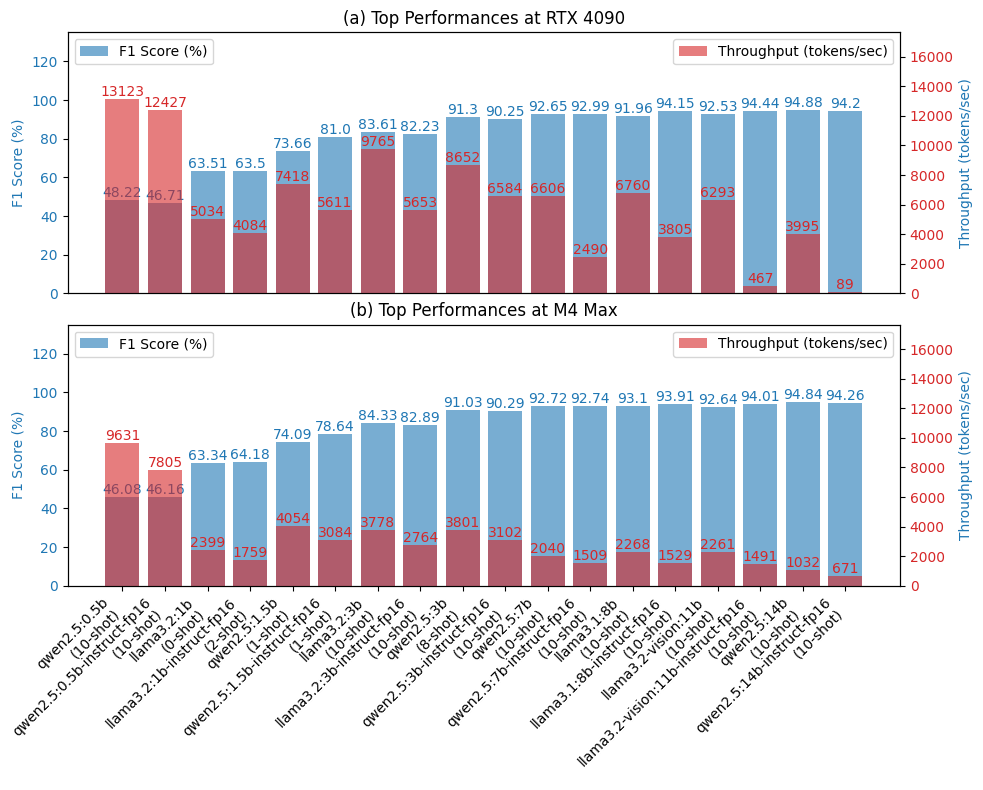
\includegraphics[width=.75\textwidth]{images/4bit_vs_fp16.png}
    \caption{Performance Comparison Between 4-bit Quantized Models and FP16 Models Across Hardware Platforms. 
    Subplot (a) displays the performance of various models on the RTX 4090 platform, while subplot (b) presents the corresponding performance on the M4 Max platform. 
    % Blue bars represent the F1 score (percentage), measured on the left y-axis, and red bars denote throughput (tokens per second), measured on the right y-axis. 
    % The x-axis labels each model with its name and the number of shots (in parentheses) that achieved the highest F1 score. 
    % Results for the 4-bit quantized variant and the FP16 variant of each model are shown side by side to facilitate direct comparison, highlighting trade-offs between accuracy and computational efficiency.
    }
    \label{fig:4bit_vs_fp16}
\end{figure*}

Fig.~\ref{fig:4bit_vs_fp16} illustrates the comparative analysis of performance and throughput across these platforms. Specifically, we examined models ranging in size from 0.5 billion to 14 billion parameters, capturing metrics such as F1 score and throughput. 

Key findings include:
\begin{itemize}
    \item Models in 4-bit precision consistently demonstrate faster evaluation times compared to FP16 across both platforms, making them highly efficient for inference tasks.
    
    \item FP16 models occasionally achieve marginally higher F1 scores—such as with smaller models like \textit{qwen2.5:1.5b}, which showed a 7.34\% improvement on the RTX 4090. However, for most models, these differences are often negligible or even negative.
    
    \item 4-bit quantization delivers significant throughput gains on both platforms, reinforcing its suitability for resource-constrained edge AI deployments.
    
    \item For larger models, such as \textit{llama3.2-vision:11b} and \textit{qwen2.5:14b}, FP16 exhibited substantial throughput reductions on both platforms, highlighting the computational efficiency of 4-bit quantization for high-demand tasks.
\end{itemize}


\begin{table}[htbp]
\centering
\begin{adjustbox}{width=0.45\textwidth}
\begin{tabular}{llrrr}
\toprule
\textbf{Model} & \textbf{\makecell{Memory\\(Load/Eval)}} & \textbf{\makecell{\% Mem.\\Reduction\\(Load/Eval)}} & \textbf{F1 (\%)} & \textbf{T-put (t/s)} \\
\midrule
\texttt{qwen2.5:0.5b} & 1.4GB/2.4GB & 30.0\%/20.0\% & 48.20 & 13,123 \\
\texttt{qwen2.5:0.5b (FP16)} & 2.0GB/3.0GB & --- & 46.70 & 12,428 \\
\cmidrule(lr){1-5}
\texttt{llama3.2:1b} & 2.8GB/5.3GB & 30.0\%/18.5\% & 63.50 & 5,035 \\
\texttt{llama3.2:1b (FP16)} & 4.0GB/6.5GB & --- & 63.50 & 4,084 \\
\cmidrule(lr){1-5}
\texttt{qwen2.5:1.5b} & 2.1GB/3.4GB & 51.2\%/39.3\% & 73.70 & 7,419 \\
\texttt{qwen2.5:1.5b (FP16)} & 4.3GB/5.6GB & --- & 81.00 & 5,611 \\
\cmidrule(lr){1-5}
\texttt{llama3.2:3b} & 4.0GB/8.2GB & 53.5\%/31.7\% & 83.60 & 9,766 \\
\texttt{llama3.2:3b (FP16)} & 8.6GB/12GB & --- & 82.20 & 5,654 \\
\cmidrule(lr){1-5}
\texttt{qwen2.5:3b} & 3.1GB/4.9GB & 58.7\%/47.3\% & 91.30 & 8,653 \\
\texttt{qwen2.5:3b (FP16)} & 7.5GB/9.3GB & --- & 90.30 & 6,584 \\
\cmidrule(lr){1-5}
\texttt{qwen2.5:7b} & 6.0GB/9.0GB & 62.5\%/52.6\% & 92.60 & 6,607 \\
\texttt{qwen2.5:7b (FP16)} & 16GB/19GB & --- & 93.00 & 2,491 \\
\cmidrule(lr){1-5}
\texttt{llama3.1:8b} & 6.7GB/11GB & 60.6\%/50.0\% & 92.00 & 6,761 \\
\texttt{llama3.1:8b (FP16)} & 17GB/22GB & --- & 94.10 & 3,805 \\
\cmidrule(lr){1-5}
\texttt{llama3.2-vision:11b} & 12GB/13GB & 52.0\%/50.0\% & 92.50 & 6,293 \\
\texttt{llama3.2-vision:11b (FP16)} & 25GB/26GB & --- & 94.40 & 468 \\
\cmidrule(lr){1-5}
\texttt{qwen2.5:14b} & 11GB/18GB & 64.5\%/52.6\% & 94.90 & 3,995 \\
\texttt{qwen2.5:14b (FP16)} & 31GB/38GB & --- & 94.20 & 89 \\
\cmidrule(lr){1-5}
\texttt{qwen2.5:32b} & 23GB/31GB & N/A & 96.90 & 2,128 \\
\cmidrule(lr){1-5}
\texttt{llama3.1:70b} & 44GB/55GB & N/A & 95.50 & 94 \\
\cmidrule(lr){1-5}
\texttt{llama3.3:70b} & 46GB/58GB & N/A & 95.70 & 73 \\
\cmidrule(lr){1-5}
\texttt{qwen2.5:72b} & 51GB/63GB & N/A & 96.90 & 109 \\
\cmidrule(lr){1-5}
\texttt{llama3.2-vision:90b} & 60GB/63GB & N/A & 96.10 & 56 \\
\bottomrule
\end{tabular}
\end{adjustbox}
\caption{Performance and resource requirements of LLMs. \texttt{FP16} refers to the FP16 precision variant of each model. “\% Mem. Reduction (Load/Eval)” shows memory savings for loading and evaluation with Q4\_K\_M quantization compared to FP16. F1 scores are percentages, and throughput (T-put) is measured in tokens per second (t/s). Metrics were collected on the RTX 4090 platform.}
\label{tab:model_memory_footprints}
\end{table}

An important consideration in the trade-offs between 4-bit quantized and FP16 models lies in their memory efficiency. Table~\ref{tab:model_memory_footprints} illustrates the significant differences in memory usage between these two precision types:

\begin{itemize}
    \item 4-bit quantized models consistently use 30.0--64.5\% less memory during loading compared to FP16. For instance, \textit{qwen2.5:1.5b} requires only 2.1GB in 4-bit versus 4.3GB in FP16. This disparity grows with model size: \textit{qwen2.5:14b} needs 11GB in 4-bit but 31GB in FP16.

    \item During evaluation, 4-bit models reduce memory usage by 20.0--52.6\%. For example, the \textit{qwen2.5:3b} model uses 4.9GB in 4-bit versus 9.3GB in FP16—a nearly 90\% increase. Interestingly, this is higher than the 9.0GB required for the evaluation of the larger \textit{qwen2.5:7b} model in 4-bit. Moreover, despite its higher memory demand, the FP16 \textit{qwen2.5:3b} performs worse, achieving a lower F1 score (90.30\% vs. 92.60\%) and reduced throughput (6,584 vs. 6,607 tokens/s).

    \item The reduced memory footprint of 4-bit models facilitates deployment on hardware with limited VRAM, such as consumer GPUs or edge devices. For instance, the \textit{qwen2.5:7b} model requires 16GB/19GB (Load/Eval) in FP16 but only 6GB/9GB in its quantized form. This makes 4-bit models practical for devices with modest memory capacities while preserving competitive performance metrics.
\end{itemize}

\subsection{Performance Analysis Across All Quantized Models}
\label{sec:all_quantized_models}

Due to hardware limitations, only the RTX A6000 [Windows], RTX A6000, RTX 4090, and M3 Max systems successfully completed the evaluation of all quantized models within a reasonable timeframe. Fig.~\ref{fig:f1_scores_all_models} presents the performance patterns across model sizes on these platforms. As the RTX A6000 [Windows] and RTX A6000 configurations produce nearly identical F1 scores across all models and shot configurations, the RTX A6000 [Windows] is excluded from this analysis.

\begin{figure*}[htbp]
    \centering
    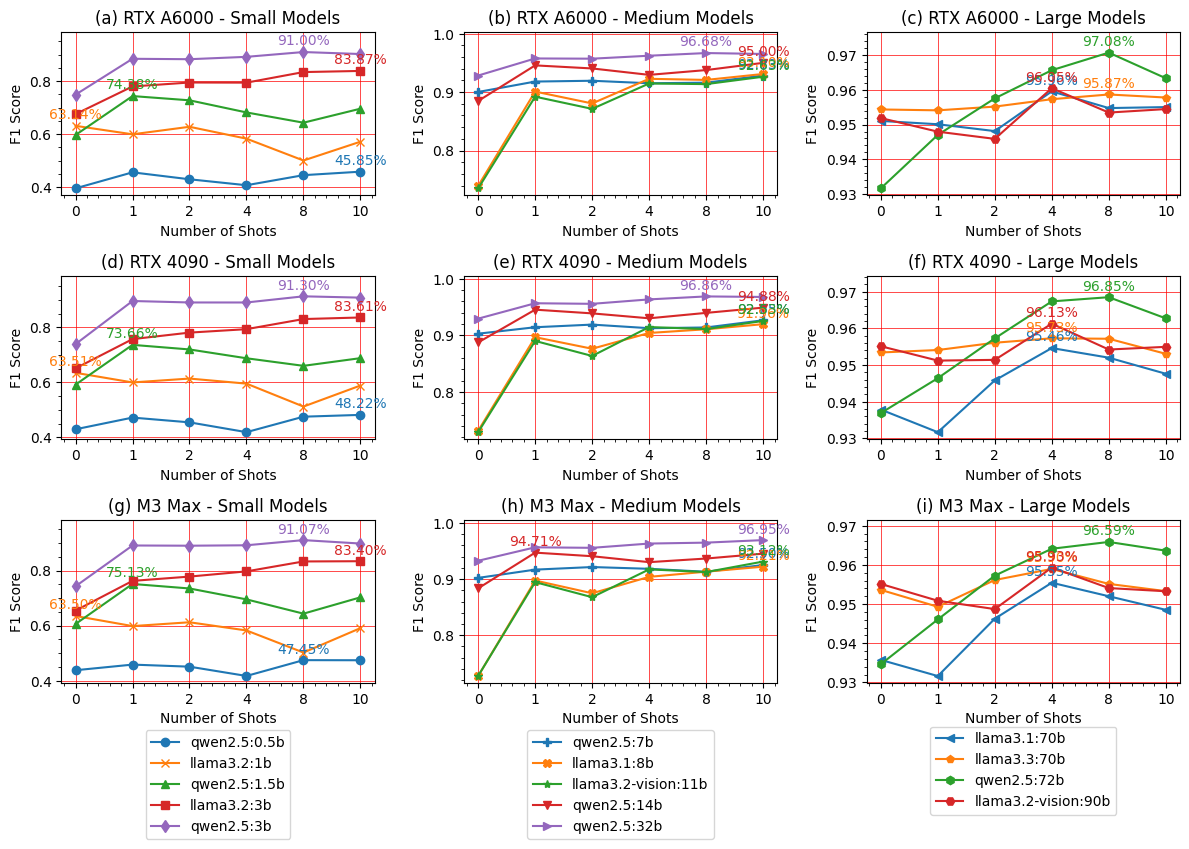
\includegraphics[width=0.8\textwidth]{images/f1_scores_all_models.png}
    \caption{F1 scores of quantized models on RTX A6000, RTX 4090, and M3 Max across different model sizes and shot counts.}
    \label{fig:f1_scores_all_models}
\end{figure*}

Our analysis reveals several key findings:

\paragraph{Small Models (0.5b--3b)} These models exhibit limited scalability with the number of shots:
\begin{itemize}
    \item Models smaller than 1.5b, such as \texttt{qwen2.5:0.5b} and \texttt{llama3.2:1b}, show modest F1 score improvements or even slight decreases across 0--10 shots, highlighting their limited few-shot learning capabilities.
    \item \texttt{qwen2.5:1.5b} achieves a notable F1 score of 73.66--75.13\% at 1 shot but exhibits diminishing returns with additional shots.
    \item Performance patterns remain consistent across all three GPU platforms.
    \item \texttt{qwen2.5:3b} achieves the highest performance among small models, reaching an F1 score of 91.00--91.30\% at 8 shots.
\end{itemize}

\paragraph{Medium Models (7b--14b)} These configurations demonstrate robust scaling:
\begin{itemize}
    \item Significant F1 score improvements are observed with few-shot learning, particularly in the 0--1 shot range.
    \item Performance remains consistent across the %RTX A6000, RTX 4090, and M3 Max 
    platforms, underscoring strong quantization robustness.
    \item \texttt{qwen2.5:32b} leads this category, achieving a remarkable F1 score of 96.68--96.95\% at 8 or 10 shots.
\end{itemize}

\paragraph{Large Models (70b--90b)} These models showcase optimal performance:
\begin{itemize}
    \item Exceptional F1 scores exceeding 95\% are achieved with as few as 4 shots.
    \item Minimal variation across GPU platforms indicates effective quantization scaling for larger models.
    \item Peak performance is achieved by \texttt{qwen2.5:72b}, reaching an impressive F1 score of 96.59--97.08\% at 8 shots.
\end{itemize}

% Across small, medium, and large models, the \texttt{qwen2.5} series consistently achieves the highest scores across these two platforms, signifying the robustness of its architecture and the effectiveness of its quantization strategy.

This analysis reveals that quantization effectively preserves model performance while enabling deployment across diverse GPU architectures. Larger models consistently outperform smaller variants, albeit at the cost of increased computational requirements. The results also highlight the effectiveness of few-shot learning in quantized settings, with most models demonstrating significant improvements within first four shots.

\subsection{Cross-Platform Performance Analysis and Hardware-Specific Insights}
\label{sec:cross-platform}

Tables~\ref{tab:small-models}, \ref{tab:medium-models}, and \ref{tab:large-models} present performance metrics under few-shot settings yielding the highest F1 scores, grouped by model size. Metrics include F1 scores, throughput (tokens/second), and mean evaluation time (seconds). Large models (70B–90B) are evaluated only on high-capacity systems (RTX A6000, RTX 4090, and M3 Max) due to memory constraints, while smaller models are tested across all platforms.

Key findings include:

\begin{enumerate}
    \item Ollama's \texttt{Q4\_K\_M} quantization outperforms bitsandbytes' 4-bit implementation. For instance, \texttt{llama3.1:8b} achieves a mean F1 score of 92.78\% ($\pm$0.50\%), surpassing its baseline of 89.50\%, while \texttt{llama3.1:70b} improves to 95.83\% ($\pm$0.07\%).
    %(Table~\ref{tab:few_shot_results}).

    \item On identical GPUs, WSL usually achieves higher throughput and lower evaluation times than Windows, particularly for smaller models. For example, on the RTX A6000, \texttt{qwen2.5:0.5b} processes 16,933 tokens/s on WSL compared to 816 tokens/s on Windows (21× faster). This gap narrows for larger models, with differences as low as 15\% at 90B. 
    %Exceptions, such as \texttt{qwen2.5:32b} on the RTX 4090 Laptop, highlight WSL's limitations under extreme memory constraints.

    \item Larger models predictably reduce throughput and increase evaluation times. For example, on the RTX 4090, throughput drops from 13,124 tokens/s (\texttt{qwen2.5:0.5b}) to 56 tokens/s (\texttt{llama3.2-vision:90b}), while evaluation time rises from 0.16 seconds to 26.505 seconds.

    \item The \texttt{qwen2.5} series consistently delivers superior F1 scores across all platforms. Notably, \texttt{qwen2.5:32b} achieves an F1 score of 96.75\% ($\pm$0.11\%) with practical inference speeds, demonstrating balanced optimization of performance and efficiency.
\end{enumerate}

% Small Models (0.5b-3b)
\begin{table}[htbp]
    \centering
    \begin{adjustbox}{width=0.4\textwidth}
    \begin{tabular}{llrrr}
\toprule
\textbf{Model} & \textbf{Platform/Stats} & \textbf{F1 (\%)} & \textbf{T-put (t/s)} & \textbf{Time (s)} \\
\midrule
\multirow[t]{10}{*}{qwen2.5:0.5b} & RTX A6000 & 45.85 & 16933 & 0.124 \\
 & RTX A6000 [Windows] & 45.85 & 816 & 2.573 \\
 & RTX 4090 & 48.22 & 13124 & 0.160 \\
 & M3 Max & 47.45 & 7178 & 0.258 \\
 & M4 Max & 46.08 & 9632 & 0.218 \\
 & RTX 4090 Laptop & 46.58 & 6907 & 0.304 \\
 & RTX 4090 Laptop [Windows] & 46.58 & 776 & 2.707 \\
 & Jetson AGX Orin & 46.65 & 1762 & 1.192 \\
 \cmidrule(lr){2-5}
 & mean & 46.66 & 7141 & 0.942 \\
 & std & 0.77 & 5561 & 1.032 \\
\cline{1-5}
\multirow[t]{10}{*}{llama3.2:1b} & RTX A6000 & 63.14 & 3922 & 0.276 \\
 & RTX A6000 [Windows] & 63.14 & 401 & 2.698 \\
 & RTX 4090 & 63.51 & 5035 & 0.215 \\
 & M3 Max & 63.50 & 1899 & 0.570 \\
 & M4 Max & 63.34 & 2400 & 0.451 \\
 & RTX 4090 Laptop & 62.65 & 1893 & 0.572 \\
 & RTX 4090 Laptop [Windows] & 62.65 & 361 & 2.998 \\
 & Jetson AGX Orin & 63.41 & 352 & 3.074 \\
 \cmidrule(lr){2-5}
 & mean & 63.17 & 2033 & 1.357 \\
 & std & 0.33 & 1622 & 1.223 \\
\cline{1-5}
\multirow[t]{10}{*}{qwen2.5:1.5b} & RTX A6000 & 74.38 & 8744 & 0.134 \\
 & RTX A6000 [Windows] & 74.38 & 456 & 2.571 \\
 & RTX 4090 & 73.66 & 7419 & 0.158 \\
 & M3 Max & 75.13 & 2224 & 0.527 \\
 & M4 Max & 74.09 & 4055 & 0.289 \\
 & RTX 4090 Laptop & 74.94 & 3768 & 0.311 \\
 & RTX 4090 Laptop [Windows] & 74.94 & 429 & 2.733 \\
 & Jetson AGX Orin & 72.16 & 740 & 1.583 \\
 \cmidrule(lr){2-5}
 & mean & 74.21 & 3479 & 1.038 \\
 & std & 0.90 & 2983 & 1.028 \\
\cline{1-5}
\multirow[t]{10}{*}{llama3.2:3b} & RTX A6000 & 83.87 & 12220 & 0.171 \\
 & RTX A6000 [Windows] & 83.87 & 803 & 2.601 \\
 & RTX 4090 & 83.61 & 9766 & 0.214 \\
 & M3 Max & 83.40 & 2521 & 0.829 \\
 & M4 Max & 84.33 & 3779 & 0.553 \\
 & RTX 4090 Laptop & 84.18 & 4850 & 0.380 \\
 & RTX 4090 Laptop [Windows] & 84.18 & 662 & 2.783 \\
 & Jetson AGX Orin & 84.34 & 596 & 3.091 \\
 \cmidrule(lr){2-5}
 & mean & 83.97 & 4400 & 1.328 \\
 & std & 0.32 & 4115 & 1.182 \\
\cline{1-5}
\multirow[t]{10}{*}{qwen2.5:3b} & RTX A6000 & 91.00 & 10118 & 0.183 \\
 & RTX A6000 [Windows] & 91.00 & 710 & 2.608 \\
 & RTX 4090 & 91.30 & 8653 & 0.214 \\
 & M3 Max & 91.07 & 1197 & 1.547 \\
 & M4 Max & 91.03 & 3802 & 0.487 \\
 & RTX 4090 Laptop & 90.65 & 4797 & 0.386 \\
 & RTX 4090 Laptop [Windows] & 90.65 & 659 & 2.808 \\
 & Jetson AGX Orin & 90.46 & 730 & 2.536 \\
 \cmidrule(lr){2-5}
 & mean & 90.89 & 3833 & 1.346 \\
 & std & 0.26 & 3537 & 1.089 \\
% \cline{1-5}
\bottomrule
\end{tabular}
    \end{adjustbox}
    \caption{Performance Metrics for Small Models (0.5b-3b). F1 scores are expressed as percentages, throughput (T-put) is measured in tokens per second (t/s), and mean evaluation time (Time) is measured in seconds (s).}
    \label{tab:small-models}
\end{table}

% Medium Models (7b-32b)
\begin{table}[htbp]
    \centering
    \begin{adjustbox}{width=0.4\textwidth}
    \begin{tabular}{llrrr}
\toprule
\textbf{Model} & \textbf{Platform/Stats} & \textbf{F1 (\%)} & \textbf{T-put (t/s)} & \textbf{Time (s)} \\
\midrule
\multirow[t]{10}{*}{qwen2.5:7b} & RTX A6000 & 92.74 & 7298 & 0.288 \\
 & RTX A6000 [Windows] & 92.83 & 784 & 2.681 \\
 & RTX 4090 & 92.65 & 6607 & 0.318 \\
 & M3 Max & 92.50 & 1194 & 1.760 \\
 & M4 Max & 92.72 & 2041 & 1.030 \\
 & RTX 4090 Laptop & 92.46 & 3944 & 0.533 \\
 & RTX 4090 Laptop [Windows] & 92.46 & 705 & 2.983 \\
 & Jetson AGX Orin & 92.78 & 410 & 5.130 \\
 \cmidrule(lr){2-5}
 & mean & 92.64 & 2873 & 1.840 \\
 & std & 0.14 & 2582 & 1.579 \\
\cline{1-5}
\multirow[t]{10}{*}{llama3.1:8b} & RTX A6000 & 93.10 & 7855 & 0.266 \\
 & RTX A6000 [Windows] & 93.10 & 778 & 2.684 \\
 & RTX 4090 & 91.96 & 6761 & 0.309 \\
 & M3 Max & 92.21 & 1430 & 1.461 \\
 & M4 Max & 93.10 & 2269 & 0.921 \\
 & RTX 4090 Laptop & 93.19 & 3935 & 0.531 \\
 & RTX 4090 Laptop [Windows] & 93.19 & 706 & 2.959 \\
 & Jetson AGX Orin & 93.10 & 406 & 5.146 \\
 \cmidrule(lr){2-5}
 & mean & 92.87 & 3017 & 1.785 \\
 & std & 0.46 & 2704 & 1.597 \\
\cline{1-5}
\multirow[t]{10}{*}{llama3.2-vision:11b} & RTX A6000 & 92.63 & 7944 & 0.263 \\
 & RTX A6000 [Windows] & 92.63 & 780 & 2.680 \\
 & RTX 4090 & 92.53 & 6293 & 0.332 \\
 & M3 Max & 93.12 & 1232 & 1.696 \\
 & M4 Max & 92.64 & 2261 & 0.924 \\
 & RTX 4090 Laptop & 93.39 & 3927 & 0.532 \\
 & RTX 4090 Laptop [Windows] & 93.39 & 707 & 2.956 \\
 & Jetson AGX Orin & 92.82 & 456 & 4.585 \\
 \cmidrule(lr){2-5}
 & mean & 92.89 & 2950 & 1.746 \\
 & std & 0.33 & 2657 & 1.447 \\
\cline{1-5}
\multirow[t]{10}{*}{qwen2.5:14b} & RTX A6000 & 95.18 & 4105 & 0.512 \\
 & RTX A6000 [Windows] & 95.00 & 728 & 2.888 \\
 & RTX 4090 & 94.88 & 3995 & 0.526 \\
 & M3 Max & 94.78 & 343 & 3.418 \\
 & M4 Max & 94.84 & 1033 & 2.035 \\
 & RTX 4090 Laptop & 95.17 & 1988 & 1.057 \\
 & RTX 4090 Laptop [Windows] & 95.09 & 638 & 3.292 \\
 & Jetson AGX Orin & 95.06 & 204 & 10.304 \\
 & mean & 95.00 & 1629 & 3.004 \\
 & std & 0.14 & 1487 & 2.971 \\
 \cmidrule(lr){2-5}
 & mean & 94.99 & 1591 & 6.191 \\
 & std & 0.16 & 1523 & 9.086 \\
\cline{1-5}
\multirow[t]{10}{*}{qwen2.5:32b} & RTX A6000 & 96.68 & 2048 & 0.906 \\
 & RTX A6000 [Windows] & 96.68 & 560 & 3.315 \\
 & RTX 4090 & 96.86 & 2128 & 0.872 \\
 & M3 Max & 96.95 & 259 & 8.131 \\
 & M4 Max & 96.86 & 143 & 12.995 \\
 & RTX 4090 Laptop & 96.68 & 221 & 8.404 \\
 & RTX 4090 Laptop [Windows] & 96.60 & 228 & 8.130 \\
 & Jetson AGX Orin & 96.68 & 95 & 19.497 \\
 & mean & 96.75 & 710 & 7.781 \\
 & std & 0.11 & 806 & 5.916 \\
% \cline{1-5}
\bottomrule
\end{tabular}
    \end{adjustbox}
    \caption{Performance Metrics for Medium Models (7b-32b). F1 scores are expressed as percentages, throughput (T-put) is measured in tokens per second (t/s), and mean evaluation time (Time) is measured in seconds (s).}
    \label{tab:medium-models}
\end{table}

% Large Models (70b-90b)
\begin{table}[htbp]
    \centering
    \begin{adjustbox}{width=0.4\textwidth}
    \begin{tabular}{llrrr}
\toprule
\textbf{Model} & \textbf{Platform/Stats} & \textbf{F1 (\%)} & \textbf{T-put (t/s)} & \textbf{Time (s)} \\
\midrule
\multirow[t]{6}{*}{llama3.1:70b} & RTX A6000 & 95.96 & 621 & 2.374 \\
 & RTX A6000 [Windows] & 95.96 & 312 & 4.724 \\
 & RTX 4090 & 95.46 & 94 & 15.657 \\
 & M3 Max & 95.55 & 120 & 12.293 \\
 \cmidrule(lr){2-5}
 & mean & 95.73 & 287 & 8.762 \\
 & std & 0.23 & 211 & 5.411 \\
\cline{1-5}
\multirow[t]{6}{*}{llama3.3:70b} & RTX A6000 & 95.87 & 937 & 1.966 \\
 & RTX A6000 [Windows] & 95.87 & 426 & 4.322 \\
 & RTX 4090 & 95.73 & 73 & 20.241 \\
 & M3 Max & 95.90 & 37 & 39.523 \\
 \cmidrule(lr){2-5}
 & mean & 95.84 & 368 & 16.513 \\
 & std & 0.07 & 362 & 15.030 \\
\cline{1-5}
\multirow[t]{6}{*}{qwen2.5:72b} & RTX A6000 & 97.08 & 515 & 3.604 \\
 & RTX A6000 [Windows] & 97.08 & 314 & 5.911 \\
 & RTX 4090 & 96.85 & 109 & 17.072 \\
 & M3 Max & 96.59 & 116 & 16.055 \\
 \cmidrule(lr){2-5}
 & mean & 96.90 & 263 & 10.660 \\
 & std & 0.20 & 167 & 5.970 \\
\cline{1-5}
\multirow[t]{6}{*}{llama3.2-vision:90b} & RTX A6000 & 96.05 & 117 & 12.611 \\
 & RTX A6000 [Windows] & 96.05 & 102 & 14.460 \\
 & RTX 4090 & 96.13 & 56 & 26.505 \\
 & M3 Max & 95.93 & 85 & 17.379 \\
 \cmidrule(lr){2-5}
 & mean & 96.04 & 90 & 17.739 \\
 & std & 0.07 & 23 & 5.339 \\
% \cline{1-5}
\bottomrule
\end{tabular}
    \end{adjustbox}
    \caption{Performance Metrics for Large Models (70b–90b). F1 scores are expressed as percentages, throughput (T-put) is measured in tokens per second (t/s), and mean evaluation time (Time) is measured in seconds (s).}
    \label{tab:large-models}
\end{table}

\subsection{Energy Efficiency in LLMs on RTX A6000}

Energy efficiency evaluates the trade-off between model performance and energy consumption. This subsection analyzes energy efficiency metrics for models running on RTX A6000, as shown in Fig.~\ref{fig:energy_efficiency}.

\begin{figure*}[h!]
    \centering
    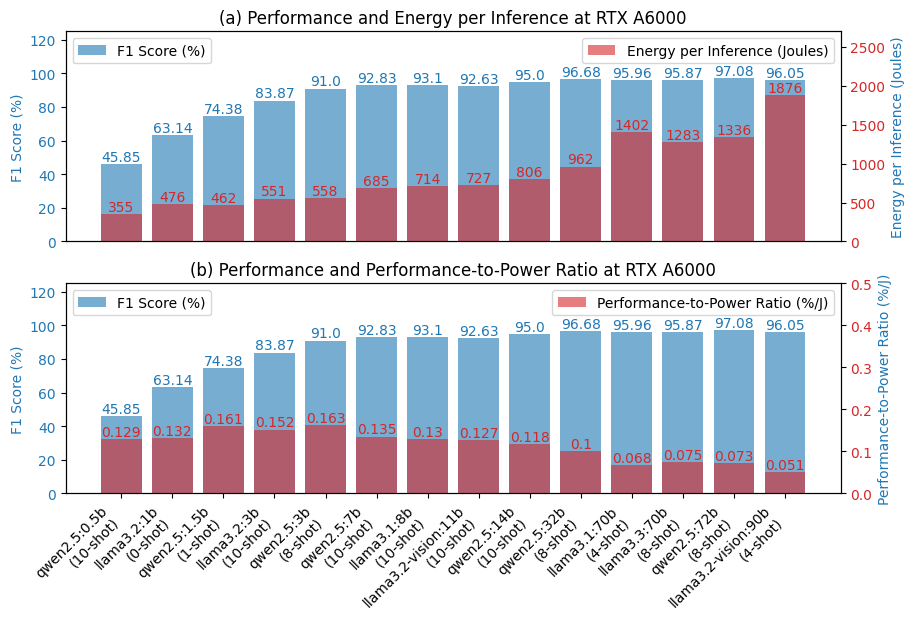
\includegraphics[width=.75\textwidth]{images/RTX-A6000-Perf-to-Power.png}
    \caption{Performance and Energy Efficiency Metrics on RTX A6000. (a) F1 Score (\%) vs. Energy per Inference (Joules). (b) F1 Score (\%) vs. Performance-to-Power Ratio (\%/J).}
    \label{fig:energy_efficiency}
\end{figure*}

Fig.~\ref{fig:energy_efficiency}(a) compare \textit{F1 Score} with \textit{Energy per Inference}:
\begin{itemize}
    \item Large models such as \texttt{qwen2.5:72b} and \texttt{llama3.2-vision:90b} achieve high F1 scores (97.08\% and 96.05\%) but consume 1,283–1,876 Joules per inference.
    \item Small models like \texttt{llama3.2-3b} and \texttt{qwen2.5:3b} consume significantly less energy (551 and 558 Joules) while achieving F1 scores of 83.87\% and 91.0\%, making them suitable for resource-constrained scenarios.
\end{itemize}

Fig.~\ref{fig:energy_efficiency}(b) highlights \textit{Performance-to-Power Ratio (\%/J)}:
\begin{itemize}
    \item Small models like \texttt{qwen2.5:1.5b} and \texttt{qwen2.5:3b} achieve the highest ratios (0.161 and 0.163 \%/J), ideal for energy-efficient deployments.
    \item Large models such as \texttt{llama3.2-vision:90b}, while achieving an F1 score of 96.05\%, have lower energy efficiency (0.051 \%/J), reflecting diminishing returns in energy usage at larger scales.
\end{itemize}

This analysis highlights the need to align model selection with deployment priorities. Large models like \texttt{qwen2.5:72b} excel in raw performance, while smaller models (\texttt{qwen2.5:1.5b} or \texttt{qwen2.5:3b}) balance performance and energy efficiency, supporting informed decision-making for diverse use cases.

% \section{Conclusion}

% This study evaluates LLMs across diverse hardware platforms using the Ollama framework, providing valuable insights into efficient edge AI deployments. Ollama’s \texttt{Q4\_K\_M} quantization outperforms bitsandbytes, with \texttt{llama3.1:8b} and \texttt{llama3.1:70b} achieving 3.28\% and 0.32\% higher F1 scores, respectively. The framework’s cross-platform stability further underscore its suitability for edge environments.

% Our findings reveal a clear relationship between model size, energy consumption, and deployment demands. Larger models exhibit improved cross-platform stability, with F1 score variances decreasing from 0.26–0.9\% (small models) to 0.07–0.22\% (large models). However, they consume up to 1,876 Joules per inference, highlighting the trade-off between raw performance and energy efficiency. Medium-sized models (7B–32B) strike a balance, with \texttt{qwen2.5:32B} achieving a 96.75\% ($\pm$0.11\%) F1 score at practical inference speeds and moderate energy consumption.

% The analysis also highlights significant efficiency gains when using Windows Subsystem for Linux (WSL), which delivers up to 21× higher throughput for smaller models compared to native Windows. These results demonstrate that energy-efficient deployments on consumer-grade GPUs are achievable with the right configurations, making edge AI accessible to a broader audience. By reducing energy consumption and infrastructure requirements, this work contributes to sustainable AI deployment. Edge computing minimizes the environmental impact of LLMs by enabling local execution, reducing reliance on energy-intensive cloud infrastructure. %Smaller models like \texttt{qwen2.5:1.5b} and \texttt{qwen2.5:3b}, with performance-to-power ratios of 0.161 and 0.163 \%/J, respectively, offer viable solutions for resource-constrained environments without compromising performance.

% To further promote socially beneficial edge AI, we propose:
% \begin{enumerate}
%     \item Developing lightweight models and quantization techniques optimized for low-cost, energy-efficient devices
%     \item Establishing benchmarks for social impact metrics such as energy efficiency, cost-effectiveness, and accessibility
%     \item Investigating edge AI solutions for humanitarian applications and disaster response scenarios
% \end{enumerate}

% This work advances the democratization of AI, enabling inclusive, sustainable, and privacy-preserving deployments that reduce environmental impact, support underserved communities, and address digital divides.

\section{Conclusion}

This study evaluates LLMs across diverse hardware platforms using the Ollama framework, offering insights into efficient and sustainable edge AI deployments. Ollama’s \texttt{Q4\_K\_M} quantization outperforms bitsandbytes, with \texttt{llama3.1:8b} and \texttt{llama3.1:70b} achieving 3.28\% and 0.32\% higher F1 scores, respectively. The framework’s cross-platform stability further underscores its suitability for edge environments.

Our results reveal a trade-off between model size, energy consumption, and performance. Larger models show increased cross-platform stability, with F1 score variances narrowing from 0.26–0.9\% (small models) to 0.07–0.22\% (large models), but at the cost of higher energy usage—up to 1,876 Joules per inference. Medium-sized models (7B–32B) offer a strong balance, with \texttt{qwen2.5:32B} achieving a 96.75\% ($\pm$0.11\%) F1 score at practical speeds and moderate energy consumption.

We also find that Windows Subsystem for Linux (WSL) can deliver up to 21× higher throughput for smaller models compared to native Windows, enabling efficient deployment on consumer-grade GPUs. These results show that, with the right configurations, energy-efficient edge AI is both feasible and accessible. By reducing infrastructure needs and supporting local execution, edge deployments can mitigate the environmental footprint of LLMs and promote more sustainable AI systems.

Future work may include:
\begin{enumerate}
    \item Validating observed performance and efficiency trends across more datasets and domains.
    \item Benchmarking Ollama’s \texttt{Q4\_K\_M} quantization against alternatives (e.g., INT8).
    \item Including broader sustainability metrics such as hardware lifecycle and total cost of ownership.
    \item Exploring practical deployment and scalability challenges through real-world case studies.
\end{enumerate}

This work advances the democratization of AI, promoting inclusive, sustainable, and privacy-preserving deployments that reduce environmental impact, empower underserved communities, and bridge digital divides.

\bibliographystyle{IEEEtran}
\bibliography{references}

\end{document}